%%%--------------------------------%%%
%%% Theory
%%%--------------------------------%%%
\section{Risk Management}
\label{sec:theoryA}
Software projects in the past have struggled to succeed. The Standish Group \cite{thestandishgroupinternationalincChaosReport20152015} has compiled a database of over 25,000 software projects over the years 2011 to 2015. They found that only about 30 percent of these projects were successful without any curtailments. The larger the projects were the less often they turned out successful. This issue has been discussed in the literature since even before the early 1990ies \cite{Boehm1991SoftwareRM}. Almost two decades later the problem of IT project failure still persists motivating this work. 

\subsection{Project Failure}
\label{sec:theorAa}
There are plenty of reasons for projects to fail and frequently even large companies and organizations experience costly failures of big projects \cite{dwivediResearchInformationSystems2015}. Projects are often defined as failed, when they cannot meet time or budget constraints or do not fulfill the pre-defined requirements. However, this definition is not useful in every context \cite{debakkerDoesRiskManagement2010}. IT projects often follow agile management techniques allowing for changes in the pre-defined scopes \cite{kusay-merkleAgilesProjektmanagementIm2018}. To allow for a wider understanding of what IT-project failure means Lyytien and Hirchheim group such failures into four different categories \cite{lyytinenInformationSystemsFailures1988}: 
\begin{itemize}
	\item Correspondence: Not meeting the pre-defined objectives
	\item Process: Exceeding time or budget restrains
	\item Interaction: Lack of end-user engagement
	\item Expectation: Inability to meet stakeholder's expectations
\end{itemize}
Each of these shortcomings can be interpreted as project failure.

\subsection{Reasons for Project Failure}
\label{sec:theorAb}	
Analogous to the variety of ways in which a project can be defined as being unsuccessful there are many reasons which can lead to any such failure. Plenty research has been done to investigate the causes of project failure \cite{guptaSystematicLiteratureReview2018}.  Events that lead to project failure can be understood as risks. Islam \cite{islamSoftwareDevelopmentRisk2011} provides the following definition for risks in an IT context:\\
"Software risk, is defined as, the possibilities of suffering a loss such as budget or schedule over-runs, customer dissatisfaction, poor quality and passive customer involvement due to an undesirable event and its consequences during the life cycle of the project."

Many such risk factors have been identified in the literature by now. Whitney and Daniels \cite{whitneyRootCauseFailure2013} as well as Tesch et al \cite{teschITProjectRisk2007} present compilations of risk factors. Based on the risks provided the following types for risk factors were derived:
 \begin{itemize}	
 	\item	Lack of support
 	\item	Resources and personnel	
 	\item	Scope and requirements	
 	\item	Technology and design	
 	\item	Communication and cooperation
 	\item	Discipline and motivation
\end{itemize}		
We group the risk factors collected by the abovementioned papers into these categories according to the following table.

\begin{table}[H]
	\centering
	\caption{Categorization of risk factors}
	\noindent\adjustbox{max width=\textwidth}{%
	\begin{tabular}{c|c|c} \toprule 
		Category  & Whitney and Daniels & Tesch et al \\ \midrule
		Lack of support	 & 
		\makecell{
			Lack of executive support/commitment\\
		}&
		\makecell{
			Lack of top management commitment to the project\\
			Lack of corporate leadership\\
		}\\ \hline
		Resources and personnel	 & 
		\makecell{
			Personnel shortfall and straining computer science abilities\\
			Shortfalls in procured components or labor\\
			Resource usage and performance \\
			Poor project team composition\\
			Inadequate technical expertise\\
		}&
		\makecell{
			Insufficient/inappropriate staffing\\
			Inadequate skills and means\\
		}\\ \hline
		Scope and requirements &
		\makecell{
			Unrealistic schedules and budgets\\
			Constantly changing requirements \\
			Unrealistic project goals and objectives\\
		}&
		\makecell{
			Lack of frozen requirements\\
			Changing scope/objectives\\
			Excessive schedule pressure\\
			Changing needs\\
			Excessive and secondary innovation\\
			Requirements creep\\
		}\\ \hline
		Technology and design &
		\makecell{
			Developing wrong functions, properties, and/or user interfaces\\
			System functionality\\
			Problematic technology base/infrastructure\\
		}&
		\makecell{
			Introduction of new technology\\
			Lack of technical specification\\
		}\\  \hline
		Communication and cooperation &
		\makecell{
			Scheduling and timing\\
			Subcontracting \\
			Personnel management\\
			Project management and control problems\\
		}&
		\makecell{
			Lack of adequate user involvement\\
			Failure to manage end user expectations\\
			Misunderstanding the requirements\\
			Conflict between user departments\\
			Poorly communicated goals/deliverables\\
			Poor project management\\
			Lack of a documented project plan\\
		} \\ \hline
		Discipline and motivation &
		\makecell{
			None\\
		}&
		\makecell{
			Failure to gain user commitment\\
			Lack of scientific methods\\
			Ignoring the obvious\\
			Unethical behavior\\
		} \\ \hline
	\end{tabular}}
	\label{tab:riskfactorscategorization}
\end{table}
To counter such risk factors risk management practices can be integrated into the overall project management. Risk management serves to identify risks, analyze them and to address them to minimize the damage these risks could do to project \cite{teschITProjectRisk2007}.

\subsection{Project Risk Management}
\label{sec:theoryAc}
Risk management is a process that should be initiated early in the project lifecycle to enable proactive handling of threats \cite{islamSoftwareDevelopmentRisk2011}. In general the cycle of risk management involves the following steps: Identification, Analysis, Response/Treatment and monitoring and control \cite{islamSoftwareDevelopmentRisk2011}, \cite{teschITProjectRisk2007}, \cite{didragaRoleEffectsRisk2013}. The steps should be undertaken at the beginning of the project and updated whenever changes occur. There are different and more detailed variations \cite{teschITProjectRisk2007}, however for the purpose of this paper the general model will be assessed in more detail.

\begin{figure}[htbp] 
	\centering
	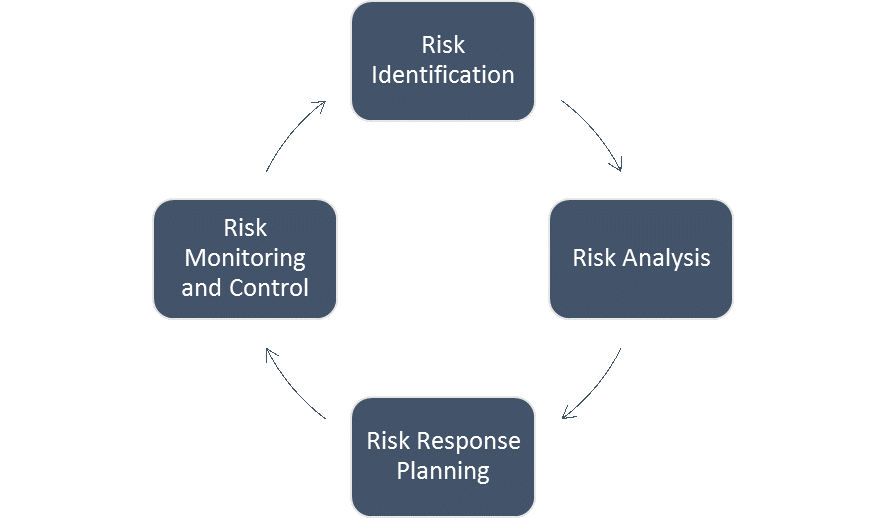
\includegraphics[width=1.0\textwidth]{Content/Theory/RiskManagementCycle.png}
	\caption{Risk Management Circle}
	\cite{own representation}
	\label{fig:riskmanagmentcycle}
\end{figure}

The different steps of the process serve different purposes and have different side effects. Risk identification helps to create awareness and to initiate action in general. It is also a phase during which the project team and stakeholders can share their concerns regarding the project and clarify their expectations to form a common view \cite{didragaRoleEffectsRisk2013}.

To actually perform the identification different techniques can be used. Two commonly used ones are the checklist and brainstorming \cite{islamSoftwareDevelopmentRisk2011}, \cite{didragaRoleEffectsRisk2013}. Checklists rely on past experience to identify known risk factory which are applicable to the project at hand. Another variant of procedure is to use a questionnaire instead which covers characteristics of the project to find specifically corresponding risks. Brainstorming is ideally done together with project stakeholders to gain different perspectives. Risk identification techniques are not mutually exclusive and combinations may result in more comprehensive results \cite{islamSoftwareDevelopmentRisk2011}.

Risk analysis serves to create acceptance of the previously identified risks as well as to indicate their impact \cite{didragaRoleEffectsRisk2013}. During this phase the likelihood of risk occurrence and the impact are estimated. This can be done in a qualitative manner by assigning ordinal values for both dimensions. The scales for likelihood can for example go from rare to almost certain. Impact can be described from low to catastrophic. Such estimates are subjective and my produce unclear results however trying to apply quantitative techniques can be unreliable as well since estimations based on past data may not be applicable anymore in a rapidly changing environment such as IT \cite{islamSoftwareDevelopmentRisk2011}.

Risk response planning serves to reduce threats and to enhance opportunities \cite{teschITProjectRisk2007}. Dealing with risks can be approached in different manners. Measurements can be defined to either avoid or prevent the risks or to deal with the impact should the risk occur. Another alternative can be to simply accept the risks or to outsource the risks \cite{islamSoftwareDevelopmentRisk2011}. Another practice used is to assign risk owners to establish clear responsibility for later control efforts \cite{peixotoProjectRiskManagement2014}.

Risk control serves to initiate action on the monitored risks and to direct action \cite{islamSoftwareDevelopmentRisk2011}. Monitoring the risks enables responding to changes via new cycles of the risk management process as well as triggering the measurements defined during the previous phase if necessary \cite{teschITProjectRisk2007}.  Techniques employed during this phase can be risk audits, trend analysis or regular status meetings \cite{islamSoftwareDevelopmentRisk2011}.
\begin{table}[H]
	\centering
	\caption{Summary effects and practices of the different phases of risk management}
	\noindent\adjustbox{max width=\textwidth}{%
\begin{tabular}{c|c|c} \toprule 
Phase  & Effects on the project & Risk management practices \\ \midrule
 Risk identification & 
 \makecell{Initiate action\\
 	Create awareness\\
 	Stakeholder communication\\
 	Common view on the project\\ 
 	Clarify expectations}&
 \makecell{Checklists\\
 	Brainstorming}\\ \hline
 Risk analysis &
 \makecell{Create acceptance \\
 	Identify risk impact\\
 	Estimate risk occurrence likelihood }&
 \makecell{Qualitative estimation\\
 	Quantitative analysis}\\ \hline
 Risk response planning &
 \makecell{Reduce threats\\
 	Enhance opportunities }&
 \makecell{Contingency plan\\
 	Risk avoidance or prevention\\
 	Risk acceptance\\
 	Outsourcing\\
 	Risk ownership }\\  \hline
 Risk monitoring and controlling &
 \makecell{Initiate and direct actions\\
 	React to changes }&
 \makecell{Risk audit\\
 	Trend analysis\\
 	Status meeting 	
 } \\ \hline
	\end{tabular}}
	\label{tab:riskmanagemensummery}
\end{table}
Different studies have been undertaken to evaluate the effect of risk management on project success \cite{debakkerDoesRiskManagement2010}, \cite{didragaRoleEffectsRisk2013}, \cite{kwakProjectRiskManagement2004}, \cite{juniorUnderstandingImpactProject2013}. The results vary regarding which part of risk management or which tools and techniques contribute to projects success but some sort of positive impact is reported from all of them.

However, in practice risk management is often neglected \cite{kwakProjectRiskManagement2004}. Even if there is initial investment into risk management during the planning phase of a project there are tendencies to let efforts slide once the project is running and time pressure picks up \cite{peixotoProjectRiskManagement2014}. Another attitude towards risk management that has been observed is to view it as additional work and cost which can hinder the adoption of any such practices \cite{teschITProjectRisk2007}.

\subsection{Conclusions for Risk Management Software}
\label{sec:theoryAd}
For the development of a software tool to facilitate risk management in IT projects the following conclusions can be drawn from the above presented:
\begin{itemize}
	\item The tool should provide functionalities for all four phases of risk management
	\item To address the project stakeholders the tool should facilitate risk management practice and provide transparency
	\item The tool should be easy to use as to speed up risk management processes
	\item The tool should be engaging to prevent negligence in times of pressure	
\end{itemize}
Further aspects to pay attention to when developing a risk management tool as presented by Keshlaf and Hashim \cite{keshlafModelPrototypeTool2000} are:
\begin{itemize}
	\item	Documentation and building on that graphical preparation and usage of the documented risks
	\item	User assistance for the risk estimation process
	\item	Versatile applicability
	\item	Comprehensiveness
	\item	Automation	
\end{itemize}

As presented above the topic of risk management in IT projects is widely covered in the literature. Risk management tools are available on the market and also discussed on a theoretical basis as seen in Keshlaf and Hashim. The novelty of this project is that we emphasize user engagement by employing gamification techniques as presented in the following chapter.